\documentclass[10pt,a4paper]{article}
\usepackage[T1]{fontenc}
\usepackage[utf8]{inputenc}
\usepackage{newtxtext,newtxmath}
\usepackage[margin=2.2cm]{geometry}
\usepackage{amsmath,booktabs,longtable,array,graphicx,microtype}
\usepackage[super,sort&compress]{natbib}
\usepackage[colorlinks=true,allcolors=teal]{hyperref}
\usepackage{placeins}
\newcommand{\CPtwoK}{CP2K}\newcommand{\Skala}{Skala}
\newcommand{\GPW}{GPW}\newcommand{\GAPW}{GAPW}\newcommand{\GTH}{GTH}
\newcommand{\GauXC}{GauXC}\newcommand{\PySCF}{PySCF}
\renewcommand{\thesection}{S\arabic{section}}
\renewcommand{\thetable}{S\arabic{table}}
\renewcommand{\thefigure}{S\arabic{figure}}
\renewcommand{\theequation}{S\arabic{equation}}
\renewcommand{\thepage}{S\arabic{page}}
\setlength{\emergencystretch}{2em}
\title{Electronic Supplementary Information\\[6pt]\large Native-grid Skala in CP2K: a GPW/GAPW route from gas-phase molecules to condensed phases}
\author{Franz P\"oschel, Johann Pototschnig,\\J\"urg Hutter, and Thomas D. K\"uhne}
\date{}
\begin{document}
\maketitle
\tableofcontents
\clearpage

\section{Scope and Notation}

The ESI documents the numerical definition and validation of the molecular and condensed-phase comparisons. Self-consistent-field (SCF) convergence, basis resolution, and grid resolution are assessed separately. Electronic occupations and the overlap-matrix trace define the explicitly treated particle number; integration on the model quadrature provides an additional discretization diagnostic. A nonzero quadrature error is therefore distinct from an incorrect occupation count. The calculations do not renormalize the model density.

GAPW-XC denotes the XC-specific augmented density decomposition, and not merely the name of an input switch. AE denotes all-electron GAPW. GTH-direct and GTH-1C denote pseudopotential GAPW evaluated with direct valence and one-centre reconstructed fields. The mixed molecular and solid protocols combine AE and GTH treatments; they are not hybrid XC functionals. AE and GAPW-XC already contain their intrinsic one-centre terms. The independent with/without comparison applies to the two ordinary pseudopotential GAPW routes.

Machine-readable reaction values, selected energy--volume curves, molecular-crystal total energies, and exact inputs are organized separately in the accompanying benchmark repository. The numerical tables below are generated from those datasets rather than transcribed from working logs.

\section{Reconstruction and Derivative Consistency}

\subsection{Spin-gradient cross terms}

Write the two reconstructed gradient fields as $\mathbf g_\alpha=\widetilde{\mathbf g}_\alpha+\mathbf g^h_\alpha-\mathbf g^s_\alpha$ and analogously for $\beta$. Their three spin invariants are $\gamma_{\alpha\alpha}=\mathbf g_\alpha^2$, $\gamma_{\beta\beta}=\mathbf g_\beta^2$, and $\gamma_{\alpha\beta}=\mathbf g_\alpha\cdot\mathbf g_\beta$. For example,
\begin{align}
\gamma_{\alpha\beta}={}&\widetilde{\mathbf g}_\alpha\cdot\widetilde{\mathbf g}_\beta
+\mathbf g^h_\alpha\cdot\mathbf g^h_\beta+\mathbf g^s_\alpha\cdot\mathbf g^s_\beta\nonumber\\
&+\widetilde{\mathbf g}_\alpha\cdot\mathbf g^h_\beta+\mathbf g^h_\alpha\cdot\widetilde{\mathbf g}_\beta
-\widetilde{\mathbf g}_\alpha\cdot\mathbf g^s_\beta-\mathbf g^s_\alpha\cdot\widetilde{\mathbf g}_\beta\nonumber\\
&-\mathbf g^h_\alpha\cdot\mathbf g^s_\beta-\mathbf g^s_\alpha\cdot\mathbf g^h_\beta.
\end{align}
The six component vectors admit $\binom{6}{2}=15$ unordered off-diagonal dot products. Three are opposite-spin products within the same smooth, hard, or soft component; twelve couple different components. Thus ``15 cross terms'' counts all off-diagonal pairs, not fifteen terms all absent from three independent spin-resolved evaluations. Separate smooth/hard/soft evaluations also combine diagonal terms with the wrong nonlinear structure. Reconstructing the fields first avoids this ambiguity and retains the nonlocal coupling of the model, which cannot be recovered by adding local algebraic corrections afterwards.

\subsection{The discrete adjoint and moving grids}

For regular-grid values $u_g$ and atom-grid interpolation coefficients $I_{ig}$,
\begin{equation}
 u_i=\sum_g I_{ig}u_g+u_i^h-u_i^s,
 \qquad
 \frac{\partial E}{\partial u_g}=\sum_i I_{ig}\frac{\partial E}{\partial u_i}.
\end{equation}
The reverse mapping uses the transpose of the forward interpolation, with the energy quadrature weights included consistently in the derivative. Hard and soft adjoints carry plus and minus signs. This applies separately to density, its Cartesian gradient components, and kinetic-energy density. At fixed orbital density matrix $P$, the explicit XC derivative for a nuclear coordinate or strain parameter $\lambda$ includes both field and geometric terms,
\begin{equation}
 \left.\frac{\partial E_{\rm xc}}{\partial\lambda}\right|_P
 =\sum_i\frac{\partial E_{\rm xc}}{\partial u_i}
         \left.\frac{\partial u_i}{\partial\lambda}\right|_P
 +\left.\frac{\partial E_{\rm xc}}{\partial\lambda}\right|_{u}.
\end{equation}
The last term encompasses explicit quadrature, partition, coordinate, and model-environment dependence. The total-energy force and stress additionally use electronic stationarity and the Gaussian-basis/overlap Pulay contributions, including cell and reciprocal-lattice dependence; the XC energy alone is not stationary in $P$. An adjoint test at fixed fields is necessary but does not replace a self-consistent total-energy finite-difference test.

\subsection{Finite-difference protocol}

For a displaced coordinate $R_{A,x}$, the central estimate is
\begin{equation}
 F^{\rm FD}_{A,x}(h)=-\frac{E(R_{A,x}+h)-E(R_{A,x}-h)}{2h}.
\end{equation}
For a homogeneous $xx$ strain, both cell and Cartesian coordinates are transformed while fractional coordinates remain fixed. In the positive-pressure stress convention,
\begin{equation}
 \sigma_{xx}^{\rm FD}(\eta)=-\frac{E(+\eta)-E(-\eta)}{2\eta\Omega}.
\end{equation}
At least two step sizes distinguish truncation error from SCF noise. An SCF threshold tightened for these checks does not change the production thresholds. A molecular coordinate-scaling virial is not a periodic stress-tensor validation, and energy agreement under symmetry reduction does not establish force equivalence after a symmetry-breaking displacement.

Self-consistent checks use one water molecule in a periodically repeated 8~\AA{} cube at Gamma, without D3, to isolate the native electronic derivatives. The grid settings are 400/60~Ry, five multigrids, and 100 radial/434 angular points. The basis/core and reconstruction definitions match the corresponding production representations. The first hydrogen is displaced along $x$ by $h=10^{-3}$ and $5\times10^{-4}$ bohr. Homogeneous $xx$ strains are $\eta=10^{-4}$ and $5\times10^{-5}$. Every perturbed calculation starts from the exact central wavefunction and converges independently to an OT residual below $10^{-9}$. All 45 executions have normal termination and zero execution/time exits. The regular-grid dimensions remain unchanged under these perturbations.

\begin{table}[htbp]
\centering\small
\caption{Signed finite-difference minus analytic derivatives. Force errors are in $\mu E_h$/bohr and stress errors in MPa. Columns give the two displacement/strain steps.}
\label{tab:derivatives}
\begin{tabular}{lrrrr}
\toprule
Representation & $\Delta F(10^{-3})$ & $\Delta F(5\times10^{-4})$ & $\Delta\sigma(10^{-4})$ & $\Delta\sigma(5\times10^{-5})$\\
\midrule
GPW/GTH & +0.228 & +2.239 & +0.038 & -0.208 \\
GAPW-XC/GTH & -0.377 & +2.380 & +0.012 & -0.332 \\
GAPW-AE & +2.855 & -2.404 & +0.007 & -0.472 \\
GAPW-GTH direct & +0.212 & +1.414 & +0.044 & -0.185 \\
GAPW-GTH one centre & -2.726 & -1.977 & -0.032 & -0.017 \\
\bottomrule
\end{tabular}
\end{table}

These checks test the self-consistent total-energy derivative, including the reconstruction and moving-grid terms, rather than only model differentiation at fixed fields. The smaller steps do not uniformly reduce the error: subtraction of converged energies amplifies finite SCF and numerical noise. Consequently, no ideal quadratic step-size scaling is claimed. The test covers one Cartesian force component and one diagonal strain component in this periodic Gamma-point system. It is not a validation of every force component, shear strain, finite-k-point derivative, or symmetry-breaking displacement under point-group reduction. Exact inputs, outputs, timing records, and file/model/binary hashes accompany the machine-readable analysis.

\FloatBarrier

\section{Molecular Numerical Settings and Convergence}

\subsection{Basis, grid, and boundary conditions}

The 70-reaction comparison uses the UZH 2026.2 all-electron TZVPP-MOLOPT-PBE-ae basis and corresponding explicit-electron Hamiltonian where available; the GTH part uses TZV2P-MOLOPT-PBE-GTH bases and GTH-PBE potentials.\cite{Mirhosseini2026UZH,Goedecker1996} The all-GTH protocol uses GAPW-XC throughout. The mixed protocols share the light-element AE energies and use GTH for the retained heavy-element species, including Bi, Te, and I. This differs from the def2-based AE/ECP protocol in the molecular GauXC paper.

The molecule-centred cells add 25~\AA{} to each molecular Cartesian extent. Cell and Poisson periodicity are disabled and the analytic isolated-system Poisson solver is used. The production atom-composite quadrature has 100 radial points and the 434-point Lebedev rule. Plane-wave/relative cutoffs are 400/60~Ry for GAPW-XC/GTH and 640/60~Ry for the shared AE route. The executed inputs document the corresponding GTH one-centre settings. OT and diagonalization thresholds are $5\times10^{-7}$ and $5\times10^{-6}$, respectively. The threshold controls the solver residual, not an energy error in kcal~mol$^{-1}$.

Basis/core changes must be kept distinct from quadrature refinement. The reported AE/GTH differences are not a basis-only convergence series, and no complete-basis limit is inferred from them.

\subsection{Regular-grid cutoff}

The paired conformational test uses the same two ACONF geometries and evaluates the relative energy within each representation. The 800~Ry result of that representation is the numerical reference. The small difference between the two 800~Ry relative energies is not set to zero: convergence within a representation and agreement between representations are separate questions.

\begin{table}[htbp]
\centering\small
\caption{Conformational energy of the paired ACONF geometries in kcal mol$^{-1}$. Each error is relative to its own 800 Ry result. The relative cutoff is 60 Ry.}
\begin{tabular}{rrrrr}
\toprule
Cutoff/Ry & GPW & GAPW-XC & $\Delta$GPW & $\Delta$GAPW-XC\\
\midrule
240 & 0.774857 & 0.726730 & 0.027401 & -0.018666 \\
280 & 0.704008 & 0.739410 & -0.043448 & -0.005985 \\
320 & 0.747292 & 0.745360 & -0.000165 & -0.000035 \\
360 & 0.746783 & 0.745610 & -0.000673 & 0.000215 \\
400 & 0.749608 & 0.745215 & 0.002152 & -0.000181 \\
480 & 0.750496 & 0.745307 & 0.003039 & -0.000089 \\
560 & 0.748038 & 0.745300 & 0.000581 & -0.000095 \\
640 & 0.747593 & 0.745297 & 0.000136 & -0.000099 \\
800 & 0.747457 & 0.745395 & 0.000000 & 0.000000 \\
\bottomrule
\end{tabular}
\end{table}


At 400~Ry, the deviations from the respective 800~Ry conformational energies are $+0.002152$~kcal~mol$^{-1}$ for GPW and $-0.000181$~kcal~mol$^{-1}$ for GAPW-XC. The faster GAPW-XC convergence supports separating hard local XC structure from the smooth auxiliary grid. This is an observable-specific cutoff test, distinct from comparison with an all-electron Hamiltonian. The complete inputs and outputs accompany the table.

\subsection{Radial and angular quadrature}

\begin{table}[htbp]
\centering\small
\caption{Self-consistent GPW water quadrature test at 800/60 Ry. Total-energy shifts are relative to 200/974 and are in microhartree. Electron-integral errors refer to eight explicit electrons.}
\begin{tabular}{rrrr}
\toprule
Radial & Angular & $\Delta E/\mu E_h$ & $\Delta N/e$\\
\midrule
50 & 50 & -369.201 & +4.486e-04 \\
50 & 100 & +237.729 & -4.318e-05 \\
50 & 194 & +263.762 & -8.268e-06 \\
50 & 302 & +307.424 & -1.074e-06 \\
50 & 434 & +245.349 & -1.215e-07 \\
100 & 50 & -592.561 & +4.491e-04 \\
100 & 100 & -10.739 & -4.333e-05 \\
100 & 302 & +72.144 & -8.919e-07 \\
100 & 434 & +8.379 & -3.031e-07 \\
100 & 590 & +6.084 & -2.206e-07 \\
150 & 434 & +12.627 & -1.352e-07 \\
150 & 590 & +10.143 & -2.079e-07 \\
150 & 770 & +14.433 & -1.869e-07 \\
200 & 590 & +11.319 & -2.275e-07 \\
200 & 770 & +15.822 & -1.715e-07 \\
200 & 974 & +0.000 & -1.347e-07 \\
\bottomrule
\end{tabular}
\end{table}


The water test refines radial and angular integration independently of the plane-wave representation. The electron integral is retained as a diagnostic, without rescaling the density. Neither the small water total-energy differences nor the conformational cutoff differences define a universal reaction-energy error bound. Frozen-density calculations that did not satisfy the stated SCF acceptance are not used as converged-energy evidence.

\subsection{Molecular cell padding}

Selected matched isolated-system calculations tested added extents of 22, 24, and 25~\AA{}. The maximum species-energy changes are 0.159, 0.189, and 0.348~$\mu E_h$ for 22--24, 24--25, and 22--25~\AA{}, respectively. The corresponding maximum reaction-energy changes are 0.000138, 0.000163, and 0.000298~kcal~mol$^{-1}$. Maximum changes of the atom-grid electron integral are $7.94\times10^{-8}$, $1.43\times10^{-7}$, and $9.72\times10^{-8}$ electrons. These comparisons retain the nonperiodic analytic electrostatic treatment; old periodic or differently centred cells are not pooled with the final molecular data.
\FloatBarrier

\section{Molecular Reaction Data and Cross-Code Comparisons}

The common set contains 70 reactions from 36 parent subsets of dietGMTKN55.\cite{Gould2018,Goerigk2017} Each reaction has complete accepted species energies in every compared protocol. The remaining cases required longer SCF convergence; the final common set is fixed across methods. No additional reaction is removed on the basis of its reference error. The reaction index and source records in the repository define the selection explicitly.

The same D3 contribution is used in the native reaction comparison. Signed errors are calculation minus the official reference, and MAEs are unweighted averages over the fixed common set. They are not full-100 dietGMTKN55 statistics or WTMAD-2 values. The ozone-containing W4-11/138 reaction remains included, despite its large GTH error; it contributes 58.8\% of the all-GTH squared error. Removing it would lower the 69-reaction GAPW-XC MAE to 2.563~kcal~mol$^{-1}$; this is an influence diagnostic, not the headline result. The direct/one-centre mixed comparison shares all light-element AE energies, and only one retained reaction changes by more than $10^{-9}$~kcal~mol$^{-1}$.

{\small
\begin{longtable}{llrrrr}
\caption{Complete common-set reaction energies in kcal mol$^{-1}$. Ref. denotes the official reference. GX is GAPW-XC/GTH, HD/HOC the mixed direct/one-centre protocols. No reference-error outlier is omitted.}\\
\toprule
Subset & Reaction & Ref. & GX & HD & HOC\\
\midrule
\endfirsthead
\toprule
Subset & Reaction & Ref. & GX & HD & HOC\\
\midrule
\endhead
ACONF & 2 & 0.61400 & 0.30663 & 0.68210 & 0.68210 \\
ACONF & 5 & 0.59500 & 0.30757 & 0.58761 & 0.58761 \\
ACONF & 8 & 1.17800 & 0.77590 & 1.22152 & 1.22152 \\
ADIM6 & 2 & 1.99000 & 2.72718 & 2.08787 & 2.08787 \\
AHB21 & 1 & -17.79000 & -22.18751 & -20.29619 & -20.29619 \\
AHB21 & 15 & -8.62000 & -11.59294 & -10.86032 & -10.86032 \\
Amino20x4 & 23 & 4.04500 & 3.68879 & 4.42456 & 4.42456 \\
Amino20x4 & 48 & 0.54000 & 0.27631 & 0.90052 & 0.90052 \\
Amino20x4 & 56 & 1.88900 & 1.93478 & 1.58118 & 1.58118 \\
BH76 & 6 & 17.80000 & 18.56504 & 17.86395 & 17.86395 \\
BH76 & 18 & 2.50000 & -8.63844 & -1.27459 & -1.27459 \\
BH76RC & 16 & 13.40000 & 10.89326 & 13.59788 & 13.59788 \\
BHPERI & 1 & 35.30000 & 33.09940 & 39.25014 & 39.25014 \\
BHPERI & 17 & 13.10000 & 10.81645 & 12.70129 & 12.70129 \\
BHPERI & 23 & 27.80000 & 28.29192 & 26.47568 & 26.47568 \\
BHPERI & 26 & 31.30000 & 31.40095 & 30.85649 & 30.85649 \\
BHROT27 & 1 & 2.73000 & 2.69043 & 2.83649 & 2.83649 \\
BHROT27 & 10 & 8.03000 & 8.43958 & 8.00707 & 8.00707 \\
BSR36 & 4 & 8.85000 & 8.44034 & 8.81562 & 8.81562 \\
BSR36 & 21 & 9.78000 & 8.34085 & 8.82335 & 8.82335 \\
BUT14DIOL & 28 & 2.83000 & 2.69982 & 4.33282 & 4.33282 \\
BUT14DIOL & 39 & 3.10000 & 3.11306 & 4.93629 & 4.93629 \\
BUT14DIOL & 63 & 4.31000 & 4.09728 & 5.97195 & 5.97195 \\
CARBHB12 & 3 & 2.42100 & 2.69672 & 3.68798 & 3.68798 \\
CARBHB12 & 4 & 9.96700 & 9.97430 & 15.57723 & 15.57723 \\
CARBHB12 & 6 & 3.02100 & 2.95159 & 5.16892 & 5.16892 \\
CARBHB12 & 11 & 3.24100 & 3.92467 & 3.06786 & 3.06786 \\
CDIE20 & 2 & 4.40000 & 4.48598 & 4.99901 & 4.99901 \\
CDIE20 & 14 & 4.40000 & 4.56044 & 4.54726 & 4.54726 \\
CHB6 & 1 & -34.43000 & -33.49431 & -34.18723 & -34.18723 \\
DC13 & 6 & -25.70000 & -32.03193 & -31.81763 & -31.81763 \\
DC13 & 12 & -58.70000 & -60.73559 & -67.15589 & -67.15589 \\
FH51 & 25 & -20.27000 & -21.62745 & -19.42107 & -19.42107 \\
G21EA & 5 & 17.30000 & -1.42565 & 10.29928 & 10.29928 \\
G21EA & 25 & 54.70000 & 50.95114 & 51.72694 & 51.72694 \\
G21IP & 28 & 243.70900 & 239.85434 & 243.88740 & 243.88740 \\
G2RC & 15 & -39.43000 & -40.17337 & -44.40802 & -44.40802 \\
HAL59 & 21 & 10.54000 & 12.10722 & 9.89950 & 9.89950 \\
HEAVY28 & 5 & 0.98000 & 2.32113 & 1.35292 & 1.35483 \\
ICONF & 16 & 3.66000 & 4.07657 & 3.99415 & 3.99415 \\
IL16 & 3 & -116.91000 & -116.64846 & -119.94685 & -119.94685 \\
INV24 & 12 & 10.30000 & 11.08966 & 10.79061 & 10.79061 \\
INV24 & 19 & 6.20000 & 5.46217 & 6.10591 & 6.10591 \\
INV24 & 22 & 27.20000 & 27.35357 & 27.74964 & 27.74964 \\
ISO34 & 12 & 45.65000 & 48.13511 & 45.85998 & 45.85998 \\
ISOL24 & 13 & 33.02000 & 34.47575 & 34.65021 & 34.65021 \\
MB16-43 & 4 & 356.84810 & 320.43581 & 358.96453 & 358.96453 \\
MCONF & 7 & 2.92000 & 3.11166 & 2.61484 & 2.61484 \\
MCONF & 22 & 5.31000 & 5.83140 & 4.73929 & 4.73929 \\
MCONF & 30 & 4.86000 & 5.03309 & 5.16786 & 5.16786 \\
MCONF & 42 & 7.32000 & 8.16255 & 7.33699 & 7.33699 \\
PArel & 3 & 2.94000 & 2.90267 & 3.05754 & 3.05754 \\
PArel & 5 & 7.19000 & 8.68203 & 7.75014 & 7.75014 \\
PArel & 10 & 2.98000 & 2.64094 & 2.92259 & 2.92259 \\
PArel & 20 & 2.15000 & 1.17708 & 1.12222 & 1.12222 \\
PNICO23 & 13 & 3.98000 & 4.16981 & 4.46224 & 4.46224 \\
PNICO23 & 17 & 7.10000 & 7.39778 & 7.31551 & 7.31551 \\
RG18 & 1 & 0.08000 & 0.17488 & 0.13391 & 0.13391 \\
RG18 & 15 & 0.24000 & 0.48594 & 0.28332 & 0.28332 \\
S66 & 11 & 5.42000 & 5.85282 & 5.96275 & 5.96275 \\
S66 & 17 & 17.18000 & 17.67587 & 19.17660 & 19.17660 \\
S66 & 24 & 2.82000 & 3.50720 & 3.46501 & 3.46501 \\
S66 & 45 & 1.75000 & 2.59070 & 2.03582 & 2.03582 \\
SCONF & 10 & 5.65000 & 6.09695 & 8.67396 & 8.67396 \\
SIE4x4 & 7 & 31.30000 & 45.77575 & 51.75030 & 51.75030 \\
W4-11 & 136 & 126.38500 & 92.90307 & 129.75705 & 129.75705 \\
W4-11 & 138 & 147.42800 & 78.94035 & 156.69640 & 156.69640 \\
WATER27 & 17 & 76.50000 & 76.32827 & 82.77137 & 82.77137 \\
WATER27 & 20 & 26.60000 & 29.31104 & 33.76403 & 33.76403 \\
YBDE18 & 1 & 57.17000 & 55.99377 & 60.22366 & 60.22366 \\
\bottomrule
\end{longtable}
}


\subsection{Direct comparison with the previous molecular implementation}

The intersection with the archived GauXC GPW-GTH reaction data contains 65 reactions. On exactly this intersection, the MAEs against the official reference are 2.2193~kcal~mol$^{-1}$ for native GAPW-XC/GTH, 2.1811 for GauXC GPW-GTH, and 1.7800 for either native mixed protocol. Native GAPW-XC minus GauXC has mean signed difference $-0.2248$, mean absolute difference 0.4624, RMS difference 0.7797, and maximum absolute difference 3.9448~kcal~mol$^{-1}$. The largest pairwise difference is DC13/6. These values include the common dispersion convention of the archived comparison.

The prior GauXC manuscript's updated primary AE/ECP--PySCF comparison comprises all 100 reactions, not these 65 or 70.\cite{Poeschel2026MolecularSkala} The online author manuscript synchronized on 9 September 2026 reports the values in Table~\ref{tab:gauxc-context}. They supersede earlier draft aggregates and differ from the first arXiv version. The primary PySCF calculation disables the atomic-radius adjustment in Becke partitioning; using the default Bragg-radii adjustment increases its cross-code differences. This is quadrature sensitivity, not a change in the reference reaction energies.

\begin{table}[htbp]
\centering
\caption{Context from the updated 100-reaction molecular GauXC manuscript. These aggregates are quoted for their original set, not rescored or compared as if they belonged to the native 70-reaction set. Energies are in kcal~mol$^{-1}$.}
\label{tab:gauxc-context}
\begin{tabular}{lrr}
\toprule
Metric & CP2K/GauXC AE/ECP & Microsoft PySCF/Skala\\
\midrule
MAE against reference & 1.255 & 1.243\\
WTMAD-2 & 3.486 & 3.459\\
\bottomrule
\end{tabular}
\par\smallskip
Direct cross-code MAD: 0.058; signed-error $R^2$: 0.998; all absolute cross-code residuals below 0.5.
\end{table}

The difference of aggregate MAEs, 0.012~kcal~mol$^{-1}$, is not the direct cross-code MAD of 0.058~kcal~mol$^{-1}$. Nor can either quantify native/GauXC equivalence under a changed basis and core treatment. Reaction-resolved primary AE/PySCF data on the native common set are not reconstructed from plots or aggregate statistics.
\FloatBarrier

\section{K-Point and Symmetry Checks}

Symmetry reduction is a change in the quadrature representation of a fixed Brillouin-zone integral. Correct weights, rotations of orbital components, and Bloch-phase conventions are required. For finite-difference forces, the perturbed geometry may have lower symmetry than the reference geometry; consistent unreduced sampling or correctly regenerated symmetry is needed. Inversion/time-reversal reduction and full point-group reduction are not interchangeable validation labels.

Seven archived controls compare complete and reduced $4^3$ meshes for C and MgO at unchanged geometry and scientific input. The K290 reduction uses 10 irreducible points from 64, at symmetry tolerance $10^{-8}$. Table~\ref{tab:symmetry} lists the absolute energy difference per reported cell. These controls establish agreement for their specific geometries, meshes, and executables; they are not a proof for all future restarts or all symmetry operations.

\begin{table}[htbp]
\centering
\caption{Selected full/reduced-grid energy checks. Residuals are the final printed SCF values; $|\Delta E|$ is in kJ~mol$^{-1}$ of simulation cells.}
\label{tab:symmetry}
\begin{tabular}{llrrr}
\toprule
System & Representation & Full SCF residual & Reduced SCF residual & $|\Delta E|$\\
\midrule
C & GAPW-XC/GTH & $3.0\times10^{-7}$ & $2.1\times10^{-7}$ & 0.0200\\
C & GAPW-AE & $8.0\times10^{-8}$ & $9.0\times10^{-8}$ & 0.0229\\
C & Mixed direct (AE here) & $8.0\times10^{-8}$ & $9.0\times10^{-8}$ & 0.0229\\
C & Mixed one centre (AE here) & $8.0\times10^{-8}$ & $9.0\times10^{-8}$ & 0.0229\\
MgO & GAPW-XC/GTH & $4.7\times10^{-7}$ & $3.6\times10^{-7}$ & 0.0291\\
MgO & Mixed direct & $2.7\times10^{-7}$ & $4.9\times10^{-7}$ & 0.0493\\
MgO & Mixed one centre & $1.4\times10^{-7}$ & $9.0\times10^{-8}$ & 0.0378\\
\bottomrule
\end{tabular}
\end{table}

The C inputs of both mixed protocols use an AE carbon basis and potential, so those rows do not constitute additional GTH validations. Mixed MgO uses GTH Mg and AE O. The molecular-crystal production uses full point-group reduction of $3^3$ meshes. The independently reported CO$_2$ $5^3$ and NH$_3$ tolerance checks below constrain sampling and approximate-symmetry sensitivity for those cases. They should not be relabelled as full-versus-reduced tests.
\FloatBarrier

\section{Molecular-Crystal Energies and Numerical Controls}
\label{sec:x23_si}

\subsection{Geometries and electronic protocol}

The crystal and gas-phase geometries are taken from Sec.~5.6 of the versioned supporting dataset arXiv:2402.13059v1 of Della Pia \emph{et al.}\cite{DellaPia2024X23} Crystal coordinates are wrapped into the supplied cells without relaxation or symmetrization. CO$_2$ and NH$_3$ have cubic cells with $a=5.624$ and 5.1305~\AA{} and four molecules each. Urea has a tetragonal cell with $a=b=5.565$, $c=4.684$~\AA{}, and two molecules. The separately supplied gas molecules are rigidly translated into centred cells whose dimensions are the molecular extents plus 25~\AA{}. They use nonperiodic cell/Poisson settings and the analytic isolated-system solver.

All four representations use Skala-1.1 Rev1 on a smoothly partitioned atom-composite quadrature with 150 radial points and the 770-point Lebedev rule. Five multigrids use cutoffs of 800/60~Ry in both phases. AE calculations use UZH 2026.2 TZVPP-MOLOPT-PBE-ae bases and explicit nuclei. GTH calculations use TZV2P-MOLOPT-PBE-GTH and GTH-PBE potentials. One-centre calculations employ the small extended expansion and accurate augmented-XC integration. The AE hard-minus-soft fields are reconstructed before the joint model evaluation. Direct and reconstructed GTH calculations share their Hamiltonian and basis.

D3(BJ) is included once, with $s_6=1$, $s_8=1.9889$, $a_1=0.3981$, $a_2=4.4211$, and interaction cutoff 20 in the executed input convention.\cite{Grimme2010DFTD3,Grimme2011D3BJ} The B3LYP parameter alias selects these damping constants, not the electronic functional. All systems are neutral restricted singlets. OT convergence is $5\times10^{-7}$. Complex k-point orbitals use IRAC with the full all-electron preconditioner. No density renormalization, energy alignment, or fitting to the reference lattice energies is applied.

Every crystal uses a Gamma-centred $3^3$ mesh with full K290 point-group reduction. With symmetry tolerance $10^{-6}$, AE and GAPW-XC give 4, 10, and 10 irreducible points for CO$_2$, NH$_3$, and urea. The GTH-direct and GTH-1C calculations use $10^{-4}$ and give 4, 4, and 6. These finite tolerances recognize near-symmetries in the decimal coordinates without moving the atoms. Their numerical sensitivity is distinct from a full-versus-reduced-grid comparison.

\subsection{Paired energies and controls}

Table~\ref{tab:x23_total_si} gives all paired total energies. We use $E_{\rm latt}=E_{\rm solid}/Z-E_{\rm molecule}$ and $1~E_h=2625.4996394799$~kJ~mol$^{-1}$. The electronic DMC references have statistical uncertainties of 0.2, 0.1, and 0.3~kJ~mol$^{-1}$ for CO$_2$, NH$_3$, and urea. Their estimated overall uncertainty is about 2~kJ~mol$^{-1}$, rather than the smaller statistical bars alone.\cite{DellaPia2024X23} Thermal and zero-point corrections to experimental sublimation enthalpies are not added to the DMC energies.

\begin{table*}[t]
\centering
\caption{Accepted total energies including D3(BJ), in hartree, and paired lattice energies in kJ\,mol$^{-1}$. Crystal energies refer to the complete cell. Extra digits support reproducibility and are not an accuracy claim.}
\label{tab:x23_total_si}
\begin{tabular}{llrrrr}
\toprule
System & Representation & $Z$ & $E_{\rm solid}$ & $E_{\rm molecule}$ & $E_{\rm latt}$ \\
\midrule
CO$_2$ & GAPW-XC--\GTH{} & 4 & -151.045238668728 & -37.747061778360 & -37.407827 \\
CO$_2$ & \GAPW{}-AE & 4 & -754.437615342695 & -188.597190183387 & -32.066940 \\
CO$_2$ & \GAPW{}--\GTH{}, direct & 4 & -151.045104012149 & -37.747040234695 & -37.376005 \\
CO$_2$ & \GAPW{}--\GTH{}, one center & 4 & -151.045343896582 & -37.747094149196 & -37.391906 \\
NH$_3$ & GAPW-XC--\GTH{} & 4 & -47.028180200438 & -11.741781495152 & -40.074458 \\
NH$_3$ & \GAPW{}-AE & 4 & -226.314440915110 & -56.564066501520 & -38.184551 \\
NH$_3$ & \GAPW{}--\GTH{}, direct & 4 & -47.028284463885 & -11.741799977614 & -40.094368 \\
NH$_3$ & \GAPW{}--\GTH{}, one center & 4 & -47.028166197256 & -11.741777335794 & -40.076187 \\
Urea & GAPW-XC--\GTH{} & 2 & -88.087642387844 & -44.000505611404 & -113.725046 \\
Urea & \GAPW{}-AE & 2 & -450.662994683326 & -225.289437740814 & -110.427467 \\
Urea & \GAPW{}--\GTH{}, direct & 2 & -88.087842193572 & -44.000575209028 & -113.804613 \\
Urea & \GAPW{}--\GTH{}, one center & 2 & -88.087646982008 & -44.000510082308 & -113.719339 \\
\bottomrule
\end{tabular}
\end{table*}

\begin{table*}[t]
\centering
\caption{Bounded numerical sensitivities in kJ\,mol$^{-1}$ per molecule. All unlisted scientific settings are held fixed. Seven accepted control executions produce six comparisons because the atom-grid refinement requires both phases.}
\label{tab:x23_controls_si}
\begin{tabular}{@{}p{0.27\textwidth}p{0.29\textwidth}p{0.25\textwidth}r@{}}
\toprule
System and representation & Change & Observable & Shift \\
\midrule
CO$_2$, GAPW-XC--\GTH{} & 150/770 to 200/974 & $\Delta E_{\rm latt}$, both phases & $+0.044554$ \\
CO$_2$, GAPW-XC--\GTH{} & 800 to 1200 Ry & $\Delta(E_{\rm solid}/Z)$ only & $-0.015499$ \\
CO$_2$, GAPW-XC--\GTH{} & $3^3$ to $5^3$ & $\Delta E_{\rm latt}$ & $+0.000391$ \\
NH$_3$, GAPW-XC--\GTH{} & Symmetry tolerance $10^{-6}$ to $10^{-4}$ & $\Delta E_{\rm latt}$ & $-0.000429$ \\
CO$_2$, GAPW-XC--\GTH{} & CPU minus CUDA & $\Delta E_{\rm latt}$ & $-0.000127$ \\
Urea, \GAPW{}-AE & CPU minus CUDA & $\Delta E_{\rm latt}$ & $-0.000379$ \\
\bottomrule
\end{tabular}
\end{table*}


For NH$_3$, CO$_2$, and urea, respectively, the absolute AE errors are 0.544, 7.170, and 16.137~kJ~mol$^{-1}$, or 1.4\%, 24.4\%, and 14.9\% of the DMC binding magnitudes. GAPW-XC/GTH gives 1.874, 8.008, and 5.225~kJ~mol$^{-1}$, or 4.9\%, 27.2\%, and 4.8\%. Thus NH$_3$ has the smallest absolute error in each representation, whereas the CO$_2$/urea ordering depends on both core treatment and the error measure. These errors describe the combined Skala--D3(BJ) protocol at the stated basis and geometry, not separate XC, dispersion, or deformation-energy components.

Refining the paired CO$_2$ quadrature from 150/770 to 200/974 changes $E_{\rm solid}/Z$ by $-0.110687$ and $E_{\rm molecule}$ by $-0.155241$~kJ~mol$^{-1}$. Their difference, $+0.044554$~kJ~mol$^{-1}$, measures the lattice-energy sensitivity. The $5^3$ crystal check uses 11 of 125 irreducible points, compared with four of 27 at $3^3$. For k-point, symmetry-tolerance, and device checks the molecule is unchanged, so the crystal shift per molecule is also the lattice-energy shift.

The accepted 1200~Ry cutoff result concerns only the CO$_2$ crystal and is not a paired binding-energy convergence test. The separate gas-phase calculation lacks a complete runtime-provenance record and is not used. CO$_2$ CPU/CUDA and urea-AE CPU/CUDA controls retain the respective executable and scientific input apart from model device selection. Their sub-0.001~kJ~mol$^{-1}$ changes constrain device effects for these cases. No complete-basis limit, BSSE correction, equilibrium volume, elastic response, or vibrational thermodynamics is inferred from the fixed-geometry energies.

\subsection{Other density-functional approximations}

Table~\ref{tab:x23-dft-context} gives published electronic lattice energies from Della Pia \emph{et al.}\cite{DellaPia2025MLIP} Their study uses hard PAW datasets, a 1000~eV cutoff, and dense system-specific k-point meshes. These are literature protocols, not same-basis native-code controls or Skala reruns.

\begin{table}[htbp]
\centering
\caption{Literature electronic lattice energies (kJ~mol$^{-1}$), transcribed from Tables S5, S8, and S22 of Ref.~\citenum{DellaPia2025MLIP}. Dispersion models are part of each method. Different geometrical and numerical protocols preclude interpreting the differences as implementation errors.}
\label{tab:x23-dft-context}
\begin{tabular}{lrrr}
\toprule
Method & CO$_2$ & NH$_3$ & Urea\\
\midrule
PBE & -6.51 & -28.24 & -73.24\\
PBE+D3 & -25.07 & -43.76 & -109.90\\
PBE+MBD & -22.74 & -42.10 & -109.11\\
revPBE+D3 & -22.60 & -38.32 & -99.88\\
SCAN+rVV10 & -31.47 & -41.69 & -113.55\\
vdW-DF2 & -32.75 & -39.70 & -103.85\\
PBE0+MBD (FHI-aims) & -23.74 & -38.99 & -109.40\\
\bottomrule
\end{tabular}
\end{table}

Bare PBE substantially underbinds, whereas dispersion-inclusive approximations have system-dependent errors. The native Skala--D3(BJ) results therefore do not exhibit an error pattern shared by every functional, and no universal ranking follows from three crystals.

The accompanying benchmark directory contains six source geometries, 24 base inputs, accepted executed inputs, and compact energy and provenance records. Calculations use CP2K revision \texttt{37aedacbb3}, with full source and host-specific executable hashes in the archive. The crystal energies and numerical-control results are retained separately.

\FloatBarrier
\section{Ten-Solid Equations of State}
\label{sec:solids}

\subsection{Structures and common fit windows}
\label{sec:solid-structures}

The selected solids are AlN, AlP, BN, BP, C, LiCl, MgO, MgS, Si, and SiC from the Goldzak set.\cite{Goldzak2022Solids} All use conventional cubic eight-atom cells. Ten initial volumes are evenly spaced from 0.90 to 1.10 times the static-lattice experimental volume. The common fit window contains the first nine volumes for AlN and AlP, ending at 1.0777778, and all ten for the other solids. The 40 method--solid comparisons derive from 36 independent curves and 352 unique energies: the AE curves for BN and C are shared by both mixed protocols. Third-order Birch--Murnaghan fits give the equilibrium lattice constant and elastic response under isotropic compression.

The comparison uses the ten solids for which consistent EOS data were available in every representation. LiF and LiH are not included. The selection is identical across protocols and was not based on the magnitude of the reference error.

\subsection{Computational details and fit stability}
\label{sec:solid-settings}

All selected points use 800/60~Ry cutoffs, 150 radial points, the 770-point Lebedev rule, and the small extended one-centre basis. All are neutral, spin-restricted calculations with UZH 2026.2 basis and potential definitions.\cite{Mirhosseini2026UZH} GAPW-AE uses TZVPP-MOLOPT-PBE-ae orbital bases and explicit core electrons for every element. GAPW-XC/GTH uses TZV2P-MOLOPT-PBE-GTH bases and the corresponding element-specific GTH-PBE potentials. In the mixed protocols, Li, B, C, N, and O retain the AE TZVPP basis, while Mg, Al, Si, P, S, and Cl use the GTH TZV2P basis. The AE one-centre reconstruction is retained in both mixed protocols. Their direct/one-centre distinction concerns the GTH fields. Every reported energy includes D3(BJ). Diagonalization and OT use residual thresholds of $5\times10^{-6}$ and $5\times10^{-7}$, respectively. Exact inputs specify the remaining dispersion and integration conventions.

The actual Gamma-centred meshes are listed in Table~\ref{tab:actual-k-meshes}. The mesh is identical across representations at each volume but can change with volume within an EOS. Consequently, a smooth fit is not by itself evidence of k-point convergence. The selected full/reduced-mesh checks in the preceding section constrain symmetry reduction for their tested cases, not all possible geometries and restarts.

Every full-window minimum is bracketed. The largest fit RMS residual is 0.674~meV per atom. Omitting one endpoint changes the fitted lattice constant by at most 0.002444~\AA{} (mixed-direct MgS, smallest-volume point omitted) and the bulk modulus by at most 9.997~GPa (GAPW-XC AlN, largest-volume point omitted). The smallest-volume point is essential to bracketing the LiCl minimum. These tests assess fit-window sensitivity. They do not measure basis or quadrature errors and are not transferable error bars for other curves.

\subsection{Basis sensitivity of structural observables}
\label{sec:solid-basis}

The ten independent AE curves contain 98 accepted TZVPP energy points. Paired five-volume QZVPP controls are available for Si, diamond, and MgO. Structural basis convergence must be assessed over volume, separately from SCF convergence and fit stability. For a basis change,
\begin{equation}
 \delta E(V)=E_{\mathrm{QZVPP}}(V)-E_{\mathrm{TZVPP}}(V),
\end{equation}
a constant $\delta E$ changes only the energy origin. Its volume dependence can instead alter the equilibrium volume, curvature, and higher derivatives that determine the elastic response. An accurate fit to a finite-basis curve therefore does not establish basis-converged lattice constants or bulk moduli.

For each solid, we compare the same five volumes, numbered 1, 3, 5, 7, and 9 in the original ten-point series. Geometry, full k-point mesh, core treatment, cutoffs, and quadrature are unchanged at each paired volume. The QZVPP calculations use full point-group reduction, through spglib for Si and diamond and the native K290 backend for MgO, and diagonalization with an SCF threshold of $5\times10^{-6}$. Same-basis checks at volume 5 reproduce the archived TZVPP energies to $1.75\times10^{-7}$~hartree for Si and $6.05\times10^{-9}$~hartree for diamond. The corresponding MgO check at volume 3 differs by $2.56\times10^{-6}$~hartree. These small differences separate the basis effect from changes in the executable and symmetry path.

\begin{table}[htbp]
\centering\small
\caption{Matched five-volume AE basis tests. Lattice constants are in \AA{} and bulk moduli in GPa. Both bases are fitted on the same five volumes. Experimental static-lattice references are from Ref.~\citenum{Goldzak2022Solids}. These three QZVPP controls do not replace the uniform ten-solid TZVPP comparison.}
\label{tab:solid-basis}
\begin{tabular}{llrr}
\toprule
Solid & Basis/reference & $a_0$ & $B_0$\\
\midrule
Si & TZVPP & 5.3747 & 100.36\\
Si & QZVPP & 5.3551 & 106.06\\
Si & Experiment & 5.4210 & 100.30\\
C & TZVPP & 3.5292 & 491.16\\
C & QZVPP & 3.5365 & 475.81\\
C & Experiment & 3.5530 & 453.30\\
MgO & TZVPP & 4.0935 & 198.84\\
MgO & QZVPP & 4.0904 & 197.45\\
MgO & Experiment & 4.1890 & 173.00\\
\bottomrule
\end{tabular}
\end{table}


The response is material dependent (Table~\ref{tab:solid-basis}). For diamond, QZVPP increases $a_0$ by 0.00735~\AA{} and lowers $B_0$ by 15.35~GPa, improving both relative to experiment. For Si, $a_0$ decreases by 0.01950~\AA{} and $B_0$ increases by 5.70~GPa, worsening both errors. MgO changes much less, with shifts of $-0.00307$~\AA{} and $-1.39$~GPa. Its lattice constant remains substantially shorter than experiment, while its bulk modulus improves slightly but remains too large. Across the sampled volumes, the span of $\delta E(V)$ is 18.64, 24.00, and 2.19~meV per atom for diamond, Si, and MgO, respectively. These nonconstant shifts explain why the basis changes affect the fitted structure as well as the absolute energy.

All three five-point minima are bracketed, and the fit RMS residuals remain below 0.19~meV per atom. Omitting either endpoint from a QZVPP fit changes $a_0$ by at most 0.000168~\AA{} for diamond and 0.00165~\AA{} for Si. The corresponding maximum changes in $B_0$ are 5.12 and 8.25~GPa. For MgO, omitting the largest-volume point changes $a_0$ by only 0.000066~\AA{} and $B_0$ by 1.36~GPa. Its smallest-volume point is required to bracket the minimum and is retained in the reported fit. These are fit-window sensitivity measures, not uncertainty estimates. The pressure derivative is more sensitive to these sparse windows and is not used to infer an improved QZVPP prediction. The same-five-volume TZVPP fits reproduce the original ten-volume values within 0.00061~\AA{} and 0.20~GPa, so changing the fit population alone does not account for the basis shifts.

For Si, five additional QZVPP calculations at volumes 2, 4, 6, 8, and 10 complete the original ten-volume series; the five existing QZVPP energies and all TZVPP energies are reused. The added points retain the matched geometry, $4\times4\times4$ mesh, full spglib reduction to ten irreducible points, and the numerical settings above. Table~\ref{tab:si-eos-extension} compares both bases on identical fit windows. The full ten-point fits give $a_0=5.37404$ and 5.35467~\AA{} and $B_0=100.56$ and 106.89~GPa for TZVPP and QZVPP, respectively. The QZVPP shifts of $-0.01938$~\AA{} and $+6.33$~GPa confirm the increased contraction and stiffness relative to the static-lattice reference, 5.421~\AA{} and 100.3~GPa. Fit RMS residuals are 0.350 and 0.403~meV per atom.

Omitting the smallest, largest, or both endpoint volumes leaves every minimum bracketed and preserves the direction of both basis shifts. Across these windows and the full ten-point QZVPP fit, $a_0$ spans 5.35467--5.35589~\AA{}, whereas $B_0$ spans 106.04--112.69~GPa. Thus the additional sampling supports the structural trend but does not remove curvature sensitivity to the chosen fit window. These spans are not statistical uncertainty estimates, and $B'_0$ remains exploratory. Only Si has been extended to ten QZVPP volumes; diamond and MgO retain their five-volume controls.

\begin{table}[htbp]
\centering\small
\caption{Matched Si EOS fits with different sampling and fit windows. Lattice constants are in \AA{}, bulk moduli in GPa, and fit RMS residuals in meV per atom. All minima are bracketed. Five new QZVPP points complete the ten-volume curve; the original five QZVPP points and all TZVPP energies are reused. The uniform ten-solid statistics are unchanged.}
\label{tab:si-eos-extension}
\begin{tabular}{lcrrrr}
\toprule
Window & Basis & $N$ & $a_0$ & $B_0$ & RMS\\
\midrule
Original five & TZVPP & 5 & 5.37465 & 100.36 & 0.153\\
Original five & QZVPP & 5 & 5.35515 & 106.06 & 0.181\\
All ten & TZVPP & 10 & 5.37404 & 100.56 & 0.350\\
All ten & QZVPP & 10 & 5.35467 & 106.89 & 0.403\\
Omit smallest & TZVPP & 9 & 5.37395 & 104.44 & 0.173\\
Omit smallest & QZVPP & 9 & 5.35548 & 112.69 & 0.174\\
Omit largest & TZVPP & 9 & 5.37510 & 100.55 & 0.244\\
Omit largest & QZVPP & 9 & 5.35573 & 106.04 & 0.298\\
Omit both endpoints & TZVPP & 8 & 5.37458 & 103.53 & 0.098\\
Omit both endpoints & QZVPP & 8 & 5.35589 & 111.13 & 0.101\\
\bottomrule
\end{tabular}
\end{table}


The paired molecular-crystal and ice tests identify substantial basis contributions to crystal--molecule energy differences. Their magnitudes cannot be transferred directly to structural observables, which contain no gas-phase reference. The Si, diamond, and MgO controls likewise do not establish basis convergence for all ten solids. The uniform ten-solid comparison below therefore retains its original TZVPP AE protocol. The shared BN and C curves are counted once and do not constitute independent basis checks.

\subsection{Representation and material trends}
\label{sec:solid-trends}

All native lattice constants are below the static-lattice experimental reference. LiCl contracts most, by approximately 0.154--0.164~\AA{}, while C and BN contract by about 0.015--0.026~\AA{}. MgS is also strongly contracted. The common sign spans diamond, zincblende, and rocksalt structures rather than a single bonding class.

GAPW-XC and AE differ on average by 0.01893~\AA{} in $a_0$ and 10.55~GPa in $B_0$, but this comparison changes basis and core treatment as well as density representation. At fixed mixed-core Hamiltonian, the one-centre correction changes $a_0$ by 0.000135~\AA{} on average and at most 0.000542~\AA{} (AlP). The corresponding changes in $B_0$ average 1.11~GPa and reach 5.75~GPa (MgO). Excluding the two shared AE curves gives mean changes of 0.000169~\AA{} and 1.39~GPa over eight independent pairs. The main contraction trend is therefore insensitive to this representation choice.

Curvature errors are less uniform. GAPW-XC underestimates the Si bulk modulus, 92.76 versus 100.3~GPa, despite a contracted lattice, whereas AE gives 100.56~GPa. For C, GAPW-XC is closer to the reference modulus than AE. A shorter equilibrium lattice does not necessarily imply a larger bulk modulus, and AE does not improve every property of every material. Neither $a_0$ nor $B_0$ determines a cohesive energy without atomic references.

\subsection{Matched literature comparisons}
\label{sec:solid-literature}

All methods are compared against the same primary static-lattice experimental values from Goldzak \emph{et al.}\cite{Goldzak2022Solids} Their Hartree--Fock (HF), second-order M{\o}ller--Plesset perturbation theory (MP2), spin-component-scaled MP2 (SCS-MP2), and scaled opposite-spin MP2 (SOS-MP2) results cover all ten selected solids. Zhang \emph{et al.}\cite{Zhang2018Solids} supply local-density approximation (LDA), PBE, PBEsol, M06-L, SCAN, and HSE06 values for nine, excluding AlN. We use their uncorrected static electronic values, not predictions with zero-point corrections. Their SCAN calculations were non-self-consistent on PBE densities. Schimka \emph{et al.}\cite{Schimka2011HSEsol} provide PBE, PBEsol, HSE06, and HSEsol lattice constants for nine, excluding MgS. No missing bulk modulus is inferred. Self-consistent Tao--Mo results\cite{Mo2017Solids} cover eight, excluding AlN and BN, and are rescored against the same Goldzak reference.

Our periodic GFN manuscript\cite{Alizadeh2026PeriodicGFN2} supplies GFN1-xTB and GFN2-xTB lattice constants for nine shared solids, but no bulk moduli in the curated comparison table. Its ten-material set excludes MgO and LiH, whereas the present set excludes LiF and LiH. The two ten-material selections must therefore not be treated as identical.

SCS-MP2 and SOS-MP2 give matched ten-solid lattice MAEs of 0.0125 and 0.0149~\AA{}, and bulk-modulus MAEs of 4.10 and 3.88~GPa. The native ranges are 0.0728--0.0844~\AA{} and 16.61--21.77~GPa. Established semilocal and screened-hybrid methods also have smaller lattice errors on the corresponding intersections. These results identify a limitation of the present structural predictions. The comparisons do not uniquely separate functional and numerical contributions.

Alternative experimental moduli listed by Goldzak \emph{et al.} for BN, BP, and MgO are 410.2, 168.0, and 169.8~GPa, instead of the primary 388.5, 176.5, and 173.0~GPa. Simultaneously replacing all three lowers each native ten-solid modulus MAE by 1.00~GPa and leaves the qualitative conclusion intact. Broader 44-solid statistics, such as those of Tran \emph{et al.},\cite{Tran2016Solids} are not relabelled as matched ten-solid errors.

\begin{table*}[t]
\centering
\small
\caption{Selected $a_0$ values (\AA{}). Experimental references follow Ref.~\citenum{Goldzak2022Solids}. BN and C reuse the AE curve for HD and HOC. These entries are not independent calculations.}
\label{tab:selected-a0_A}
\begin{tabular}{lrrrrr}
\toprule
Solid & Experiment & GX & AE & HD & HOC \\
\midrule
AlN & 4.3680 & 4.2811 & 4.3025 & 4.2747 & 4.2746 \\
AlP & 5.4480 & 5.3622 & 5.3781 & 5.3616 & 5.3621 \\
BN & 3.5930 & 3.5777 & 3.5675 & 3.5675 & 3.5675 \\
BP & 4.5250 & 4.4439 & 4.4696 & 4.4527 & 4.4527 \\
C & 3.5530 & 3.5345 & 3.5292 & 3.5292 & 3.5292 \\
LiCl & 5.0720 & 4.9081 & 4.9155 & 4.9178 & 4.9179 \\
MgO & 4.1890 & 4.1059 & 4.0935 & 4.0923 & 4.0919 \\
MgS & 5.1880 & 5.0689 & 5.0536 & 5.0700 & 5.0697 \\
Si & 5.4210 & 5.3386 & 5.3740 & 5.3383 & 5.3383 \\
SiC & 4.3470 & 4.2517 & 4.2920 & 4.2556 & 4.2556 \\
\bottomrule
\end{tabular}
\end{table*}

\begin{table*}[t]
\centering
\small
\caption{Selected $B_0$ values (GPa). Experimental references follow Ref.~\citenum{Goldzak2022Solids}. BN and C reuse the AE curve for HD and HOC. These entries are not independent calculations.}
\label{tab:selected-B0_GPa}
\begin{tabular}{lrrrrr}
\toprule
Solid & Experiment & GX & AE & HD & HOC \\
\midrule
AlN & 206.00 & 239.07 & 225.89 & 240.42 & 240.40 \\
AlP & 87.00 & 94.34 & 101.35 & 96.36 & 93.12 \\
BN & 388.50 & 423.39 & 420.87 & 420.87 & 420.87 \\
BP & 176.50 & 187.93 & 183.64 & 185.86 & 185.86 \\
C & 453.30 & 457.33 & 491.35 & 491.35 & 491.35 \\
LiCl & 37.30 & 47.98 & 46.37 & 47.13 & 47.16 \\
MgO & 173.00 & 188.28 & 198.71 & 213.13 & 207.37 \\
MgS & 81.00 & 87.90 & 90.27 & 84.17 & 86.22 \\
Si & 100.30 & 92.76 & 100.56 & 94.13 & 94.13 \\
SiC & 228.90 & 263.89 & 241.68 & 263.73 & 263.71 \\
\bottomrule
\end{tabular}
\end{table*}

\begin{table*}[t]
\centering
\small
\caption{EOS fit diagnostics, part 1. All full-window minima are bracketed. RMS residuals are in meV per atom.}
\label{tab:eos-fit-1}
\begin{tabular}{lrrrr}
\toprule
Method & Solid & $N_V$ & $B'_0$ & RMS \\
\midrule
AE & AlN & 9 & 3.707 & 0.0418 \\
AE & AlP & 9 & 4.179 & 0.0880 \\
AE & BN & 10 & 3.772 & 0.1250 \\
AE & BP & 10 & 3.701 & 0.0311 \\
AE & C & 10 & 3.756 & 0.0542 \\
AE & LiCl & 10 & 4.029 & 0.0205 \\
AE & MgO & 10 & 4.092 & 0.0190 \\
AE & MgS & 10 & 3.682 & 0.0117 \\
AE & Si & 10 & 4.544 & 0.3496 \\
AE & SiC & 10 & 3.854 & 0.0449 \\
GX & AlN & 9 & 2.802 & 0.6739 \\
GX & AlP & 9 & 3.959 & 0.1431 \\
GX & BN & 10 & 3.713 & 0.1306 \\
GX & BP & 10 & 4.081 & 0.0723 \\
GX & C & 10 & 3.611 & 0.1734 \\
GX & LiCl & 10 & 4.027 & 0.0435 \\
GX & MgO & 10 & 3.864 & 0.2921 \\
GX & MgS & 10 & 4.349 & 0.1597 \\
\bottomrule
\end{tabular}
\end{table*}

\begin{table*}[t]
\centering
\small
\caption{EOS fit diagnostics, part 2. All full-window minima are bracketed. RMS residuals are in meV per atom.}
\label{tab:eos-fit-2}
\begin{tabular}{lrrrr}
\toprule
Method & Solid & $N_V$ & $B'_0$ & RMS \\
\midrule
GX & Si & 10 & 5.096 & 0.5702 \\
GX & SiC & 10 & 4.107 & 0.1309 \\
HD & AlN & 9 & 3.339 & 0.3028 \\
HD & AlP & 9 & 4.778 & 0.3362 \\
HD & BP & 10 & 3.918 & 0.0532 \\
HD & LiCl & 10 & 3.905 & 0.0330 \\
HD & MgO & 10 & 4.208 & 0.3562 \\
HD & MgS & 10 & 3.167 & 0.2585 \\
HD & Si & 10 & 5.257 & 0.3634 \\
HD & SiC & 10 & 4.168 & 0.0561 \\
HOC & AlN & 9 & 3.338 & 0.3027 \\
HOC & AlP & 9 & 3.787 & 0.2878 \\
HOC & BP & 10 & 3.918 & 0.0532 \\
HOC & LiCl & 10 & 3.915 & 0.0328 \\
HOC & MgO & 10 & 4.181 & 0.0393 \\
HOC & MgS & 10 & 3.865 & 0.0993 \\
HOC & Si & 10 & 5.257 & 0.3634 \\
HOC & SiC & 10 & 4.167 & 0.0557 \\
\bottomrule
\end{tabular}
\end{table*}

\begin{table*}[t]
\centering
\small
\caption{Matched comparison with Ref.~\citenum{Goldzak2022Solids}: ten-solid set. Every row uses the identical intersection and the Goldzak static-lattice experimental reference. MAE($a_0$) is in \AA{} and MAE($B_0$) in GPa. A dash denotes unavailable data, not zero error. Native rows retain the numerical qualifications discussed in the text.}
\label{tab:literature-Goldzak2022}
\begin{tabular}{lrrr}
\toprule
Method & $N$ & MAE($a_0$) & MAE($B_0$) \\
\midrule
GX & 10 & 0.0831 & 16.61 \\
AE & 10 & 0.0728 & 16.89 \\
HD & 10 & 0.0844 & 21.77 \\
HOC & 10 & 0.0844 & 21.07 \\
HF & 10 & 0.0563 & 15.23 \\
MP2 & 10 & 0.0201 & 5.71 \\
SCS-MP2 & 10 & 0.0125 & 4.10 \\
SOS-MP2 & 10 & 0.0149 & 3.88 \\
\bottomrule
\end{tabular}
\end{table*}

\begin{table*}[t]
\centering
\small
\caption{Matched comparison with Ref.~\citenum{Zhang2018Solids}: nine solids, excluding AlN. Every row uses the identical intersection and the Goldzak static-lattice experimental reference. MAE($a_0$) is in \AA{} and MAE($B_0$) in GPa. A dash denotes unavailable data, not zero error. Native rows retain the numerical qualifications discussed in the text.}
\label{tab:literature-Zhang2018}
\begin{tabular}{lrrr}
\toprule
Method & $N$ & MAE($a_0$) & MAE($B_0$) \\
\midrule
GX & 9 & 0.0827 & 14.78 \\
AE & 9 & 0.0737 & 16.56 \\
HD & 9 & 0.0834 & 20.36 \\
HOC & 9 & 0.0835 & 19.59 \\
LDA & 9 & 0.0324 & 4.66 \\
PBE & 9 & 0.0451 & 12.96 \\
PBEsol & 9 & 0.0113 & 4.72 \\
M06-L & 9 & 0.0128 & 3.46 \\
SCAN & 9 & 0.0123 & 3.08 \\
HSE06 & 9 & 0.0170 & 5.86 \\
\bottomrule
\end{tabular}
\end{table*}

\begin{table*}[t]
\centering
\small
\caption{Matched comparison with Ref.~\citenum{Schimka2011HSEsol}: nine solids, excluding MgS. Every row uses the identical intersection and the Goldzak static-lattice experimental reference. MAE($a_0$) is in \AA{} and MAE($B_0$) in GPa. A dash denotes unavailable data, not zero error. Native rows retain the numerical qualifications discussed in the text.}
\label{tab:literature-Schimka2011}
\begin{tabular}{lrrr}
\toprule
Method & $N$ & MAE($a_0$) & MAE($B_0$) \\
\midrule
GX & 9 & 0.0791 & -- \\
AE & 9 & 0.0660 & -- \\
HD & 9 & 0.0807 & -- \\
HOC & 9 & 0.0807 & -- \\
PBE & 9 & 0.0438 & -- \\
PBEsol & 9 & 0.0136 & -- \\
HSE06 & 9 & 0.0132 & -- \\
HSEsol & 9 & 0.0117 & -- \\
\bottomrule
\end{tabular}
\end{table*}

\begin{table*}[t]
\centering
\small
\caption{Matched comparison with Ref.~\citenum{Mo2017Solids}: eight solids, excluding AlN and BN. Every row uses the identical intersection and the Goldzak static-lattice experimental reference. MAE($a_0$) is in \AA{} and MAE($B_0$) in GPa. A dash denotes unavailable data, not zero error. Native rows retain the numerical qualifications discussed in the text.}
\label{tab:literature-Mo2017}
\begin{tabular}{lrrr}
\toprule
Method & $N$ & MAE($a_0$) & MAE($B_0$) \\
\midrule
GX & 8 & 0.0911 & 12.27 \\
AE & 8 & 0.0797 & 14.58 \\
HD & 8 & 0.0907 & 18.86 \\
HOC & 8 & 0.0907 & 18.00 \\
Tao-Mo & 8 & 0.0194 & 4.26 \\
\bottomrule
\end{tabular}
\end{table*}

\begin{table*}[t]
\centering
\small
\caption{Matched comparison with Ref.~\citenum{Alizadeh2026PeriodicGFN2}: nine solids, excluding MgO. Every row uses the identical intersection and the Goldzak static-lattice experimental reference. MAE($a_0$) is in \AA{} and MAE($B_0$) in GPa. A dash denotes unavailable data, not zero error. Native rows retain the numerical qualifications discussed in the text.}
\label{tab:literature-PeriodicGFN2Manuscript}
\begin{tabular}{lrrr}
\toprule
Method & $N$ & MAE($a_0$) & MAE($B_0$) \\
\midrule
GX & 9 & 0.0831 & -- \\
AE & 9 & 0.0703 & -- \\
HD & 9 & 0.0831 & -- \\
HOC & 9 & 0.0830 & -- \\
GFN1-xTB & 9 & 0.1360 & -- \\
GFN2-xTB & 9 & 0.0659 & -- \\
\bottomrule
\end{tabular}
\end{table*}

\begin{table*}[t]
\centering
\small
\caption{Actual Gamma-centered k meshes by volume index. Indices 01--10 refer to the original evenly spaced volume ratios 0.90--1.10. Each selected volume uses the same mesh in all representations, but the mesh can change along an EOS.}
\label{tab:actual-k-meshes}
\begin{tabular}{lr}
\toprule
Solid & Mesh and volume indices \\
\midrule
AlN & $5^3$: 01,02,03,04,05,06,07,08,09 \\
AlP & $4^3$: 01,02,03,04,05,06,07,08,09 \\
BN & $6^3$: 02,03,04,05,06,07,08,09,10; $7^3$: 01 \\
BP & $5^3$: 01,02,03,04,05,06,07,08,09,10 \\
C & $6^3$: 04,05,06,07,08,09,10; $7^3$: 01,02,03 \\
LiCl & $5^3$: 01,02,03,04,05,06,07,08,09,10 \\
MgO & $5^3$: 06,07,08,09,10; $6^3$: 01,02,03,04,05 \\
MgS & $4^3$: 07,08,09,10; $5^3$: 01,02,03,04,05,06 \\
Si & $4^3$: 02,03,04,05,06,07,08,09,10; $5^3$: 01 \\
SiC & $5^3$: 01,02,03,04,05,06,07,08,09,10 \\
\bottomrule
\end{tabular}
\end{table*}

\begin{figure}[htbp]
\centering
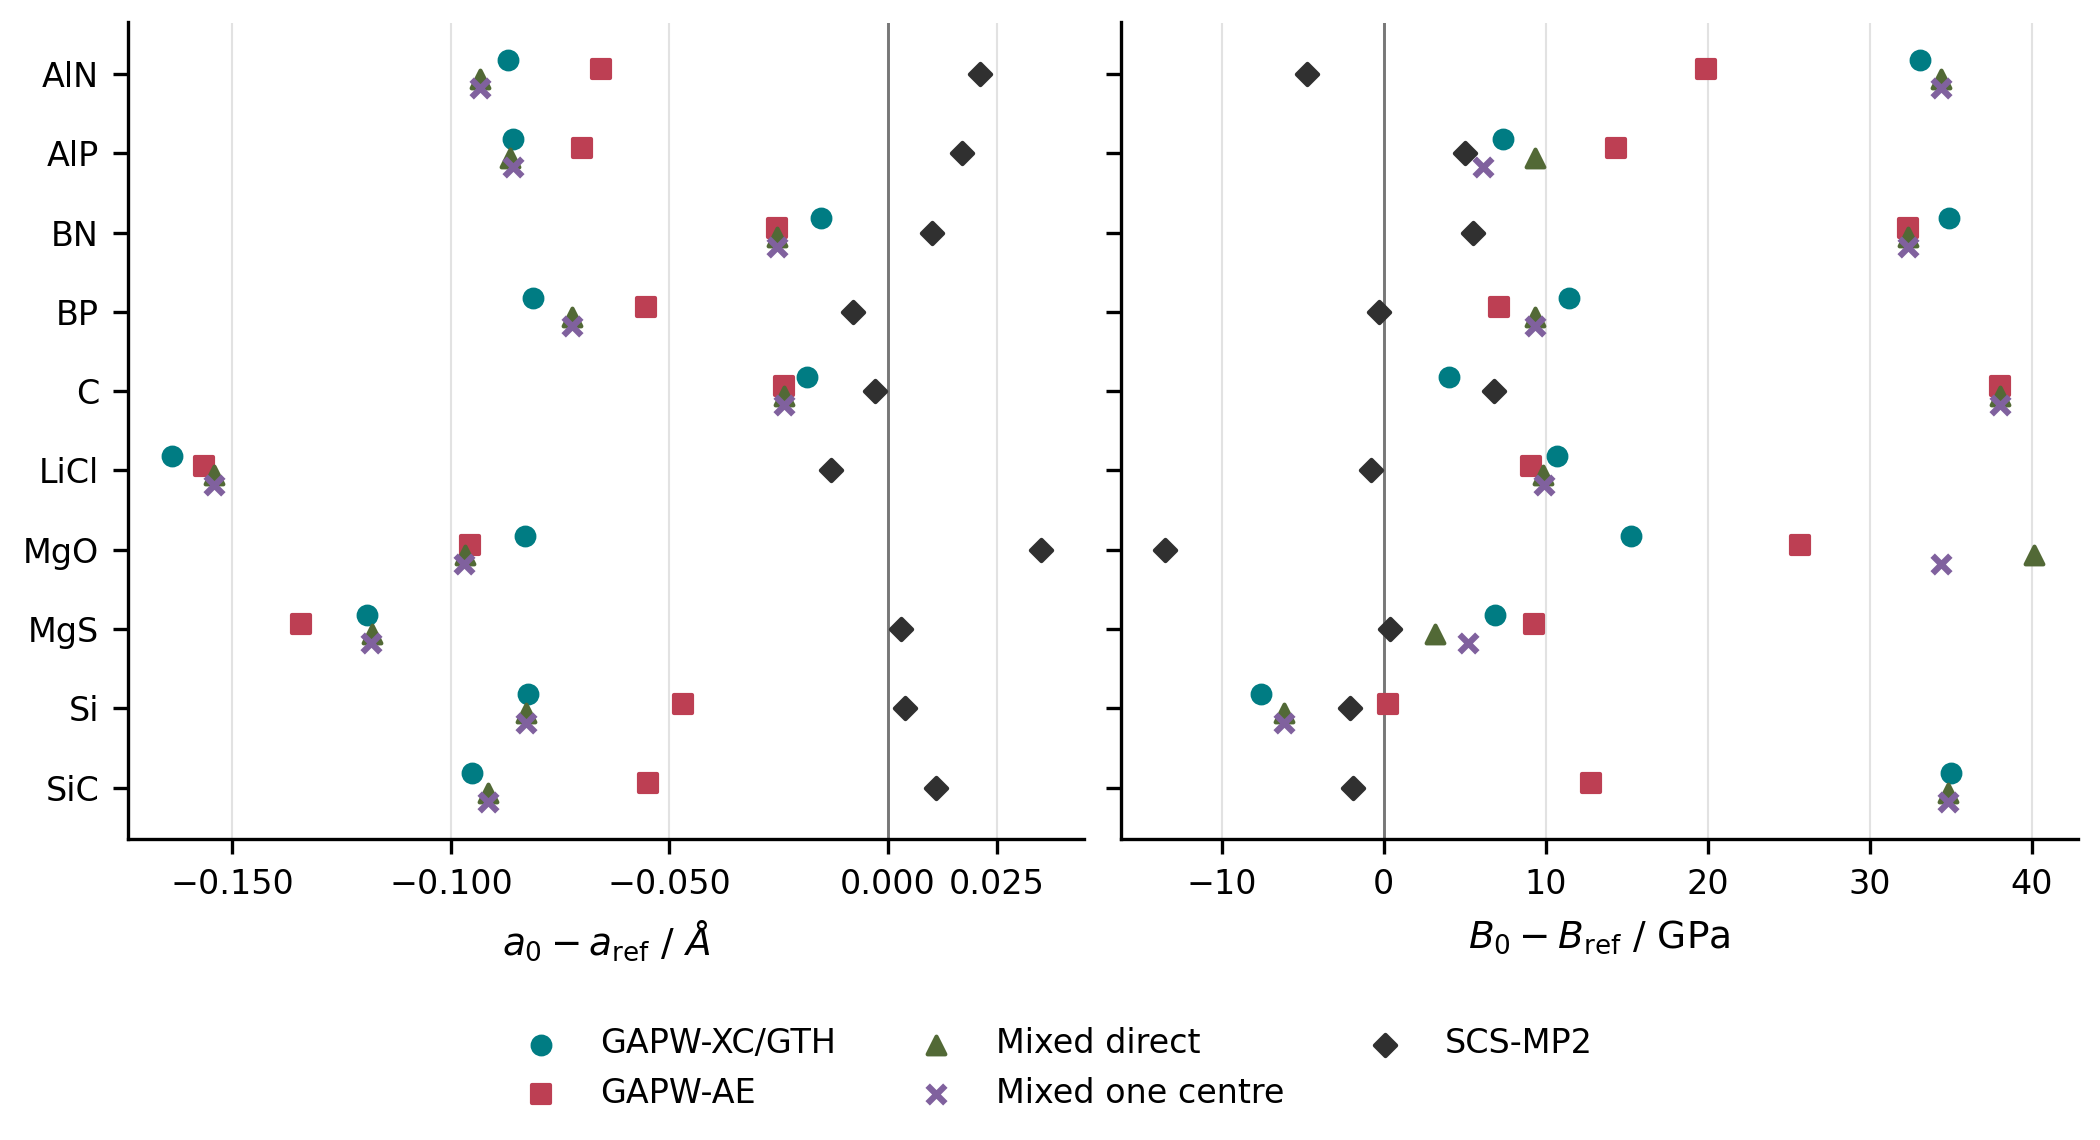
\includegraphics[width=\textwidth]{eos-literature-residuals.png}
\caption{Signed lattice-constant and bulk-modulus errors against the common Goldzak static-lattice reference. SCS-MP2 provides matched correlated-method context. Systematic native lattice contraction persists across representations. Its sign alone does not identify the source of the discrepancy.}
\label{fig:periodic-residuals}
\end{figure}

\FloatBarrier

\section{Pressure Derivatives and Compressibilities}

The third-order Birch--Murnaghan fit supplies $V_0$, $B_0$, and $B'_0=(\partial B/\partial P)_{P=0}$ in addition to $E_0$. Its energy expression is
\begin{equation}
 E(V)=E_0+\frac{9V_0B_0}{16}
 \left[B'_0(x-1)^3+(6-4x)(x-1)^2\right],\qquad
 x=(V_0/V)^{2/3}.
\end{equation}
The zero-pressure compressibility is $\kappa_0=1/B_0$. These quantities require no new SCF calculation. $B'_0$ depends on the third derivative of the fitted energy and is more sensitive to the fit interval and numerical noise than the minimum location. We therefore supplement the full-window values with endpoint-omission sensitivity rather than assigning artificial high precision from the least-squares fit.

{\small
\begin{longtable}{llrrrrr}
\caption{Additional predictions from the existing EOS data. $\kappa_0$ is in $10^{-3}$ GPa$^{-1}$; $V_0$ is the eight-atom cell volume in \AA$^3$. The endpoint column is the largest absolute change of $B_0^\prime$ after removing either endpoint. A dagger means at least one omitted-window minimum is no longer bracketed.}\\
\toprule
Method & Solid & $V_0$ & $B_0$/GPa & $B_0^\prime$ & $10^3\kappa_0$ & max. $|\Delta B_0^\prime|$\\
\midrule
\endfirsthead
\toprule
Method & Solid & $V_0$ & $B_0$/GPa & $B_0^\prime$ & $10^3\kappa_0$ & max. $|\Delta B_0^\prime|$\\
\midrule
\endhead
AE & AlN & 79.6434 & 225.89 & 3.707 & 4.427 & 0.061 \\
AE & AlP & 155.5561 & 101.35 & 4.179 & 9.867 & 0.292 \\
AE & BN & 45.4045 & 420.87 & 3.772 & 2.376 & 0.106 \\
AE & BP & 89.2889 & 183.64 & 3.701 & 5.445 & 0.050 \\
AE & C & 43.9583 & 491.35 & 3.756 & 2.035 & 0.092 \\
AE & LiCl & 118.7693 & 46.37 & 4.029 & 21.568 & 0.073$^\dagger$ \\
AE & MgO & 68.5923 & 198.71 & 4.092 & 5.032 & 0.049 \\
AE & MgS & 129.0645 & 90.27 & 3.682 & 11.077 & 0.031 \\
AE & Si & 155.2040 & 100.56 & 4.544 & 9.944 & 0.921 \\
AE & SiC & 79.0664 & 241.68 & 3.854 & 4.138 & 0.032 \\
GX & AlN & 78.4652 & 239.07 & 2.802 & 4.183 & 1.895 \\
GX & AlP & 154.1793 & 94.34 & 3.959 & 10.600 & 0.466 \\
GX & BN & 45.7944 & 423.39 & 3.713 & 2.362 & 0.129 \\
GX & BP & 87.7590 & 187.93 & 4.081 & 5.321 & 0.038 \\
GX & C & 44.1546 & 457.33 & 3.611 & 2.187 & 0.350 \\
GX & LiCl & 118.2330 & 47.98 & 4.027 & 20.844 & 0.230$^\dagger$ \\
GX & MgO & 69.2214 & 188.28 & 3.864 & 5.311 & 0.625 \\
GX & MgS & 130.2384 & 87.90 & 4.349 & 11.377 & 0.264 \\
GX & Si & 152.1509 & 92.76 & 5.096 & 10.780 & 0.810 \\
GX & SiC & 76.8604 & 263.89 & 4.107 & 3.789 & 0.230 \\
HD & AlN & 78.1094 & 240.42 & 3.339 & 4.159 & 0.634 \\
HD & AlP & 154.1285 & 96.36 & 4.778 & 10.378 & 0.750 \\
HD & BN & 45.4045 & 420.87 & 3.772 & 2.376 & 0.106 \\
HD & BP & 88.2826 & 185.86 & 3.918 & 5.380 & 0.091 \\
HD & C & 43.9583 & 491.35 & 3.756 & 2.035 & 0.092 \\
HD & LiCl & 118.9380 & 47.13 & 3.905 & 21.217 & 0.212$^\dagger$ \\
HD & MgO & 68.5343 & 213.13 & 4.208 & 4.692 & 0.337 \\
HD & MgS & 130.3228 & 84.17 & 3.167 & 11.880 & 0.631 \\
HD & Si & 152.1244 & 94.13 & 5.257 & 10.624 & 1.074 \\
HD & SiC & 77.0688 & 263.73 & 4.168 & 3.792 & 0.099 \\
HOC & AlN & 78.1082 & 240.40 & 3.338 & 4.160 & 0.634 \\
HOC & AlP & 154.1753 & 93.12 & 3.787 & 10.739 & 0.766 \\
HOC & BN & 45.4045 & 420.87 & 3.772 & 2.376 & 0.106 \\
HOC & BP & 88.2820 & 185.86 & 3.918 & 5.381 & 0.091 \\
HOC & C & 43.9583 & 491.35 & 3.756 & 2.035 & 0.092 \\
HOC & LiCl & 118.9405 & 47.16 & 3.915 & 21.203 & 0.240$^\dagger$ \\
HOC & MgO & 68.5140 & 207.37 & 4.181 & 4.822 & 0.070 \\
HOC & MgS & 130.2985 & 86.22 & 3.865 & 11.598 & 0.224 \\
HOC & Si & 152.1238 & 94.13 & 5.257 & 10.624 & 1.074 \\
HOC & SiC & 77.0679 & 263.71 & 4.167 & 3.792 & 0.099 \\
\bottomrule
\end{longtable}
}


The full-window $B'_0$ values span 2.80--5.26. The largest endpoint-induced change, 1.90, occurs for GAPW-XC AlN, whose full-window value is 2.80. This substantial sensitivity cautions against assigning physical significance to small differences between fitted pressure derivatives. The accompanying machine-readable analysis retains both endpoint tests and identifies cases in which an omitted endpoint no longer brackets the minimum.

The matched primary literature tables provide $a_0$ and $B_0$ but no consistently curated common $B'_0$ reference set. We report $B'_0$ as a derived model prediction with a fit-window diagnostic, not an accuracy ranking against an invented reference. Compressibility comparisons follow directly from the same matched $B_0$ values; they contain no independent evidence beyond that observable. The three molecular crystals have only paired single-point energies, so no bulk modulus, pressure derivative, elastic tensor, or equilibrium volume is inferred for them.

\section{Reproducibility and Numerical Limits}

The molecular, molecular-crystal, and solid subsets use distinct documented protocols and are analysed separately. Each reported energy is linked to its executed input, model and executable versions, SCF convergence, and normal termination record. Replicate calculations count once. The archive distinguishes production energies from the independent numerical controls and preserves the input and source hashes needed to reproduce the reported quantities.

The ESI reports available convergence and sensitivity data rather than claiming a universal bound on basis, integration, or k-point error. In particular, the present work does not provide complete-basis extrapolation, BSSE correction for the molecular crystals, converged phonons, finite-temperature thermodynamics, or cohesive energies for the ten solids. Such quantities would require additional calculations and reference choices. The reported lattice-energy and structural trends remain useful, provided those distinctions are maintained.

\bibliographystyle{rsc}
\bibliography{references,pccp-references,x23-references}
\end{document}
